\documentclass[10pt,a4paper]{article}
\usepackage[utf8]{inputenc}
\usepackage[T1]{fontenc}
\usepackage[french]{babel}
\usepackage{lmodern}
\usepackage[margin=2.2cm]{geometry}
\usepackage{microtype}
\usepackage{graphicx}
\usepackage{booktabs}
\usepackage{longtable}
\usepackage{tabularx}
\usepackage{array}
\usepackage{float}
\usepackage{fancyhdr}
\usepackage{xcolor}
\usepackage{hyperref}
\usepackage{enumitem}
\usepackage{setspace}
\usepackage{caption}
\usepackage{titlesec}
\usepackage{amsmath}
\usepackage{ragged2e}
\usepackage{etoolbox}
\usepackage{multicol}
\usepackage{lastpage}
\usepackage{pdfpages}

\definecolor{accent}{HTML}{163A5F}
\definecolor{softline}{HTML}{D7E2EE}
\definecolor{textgray}{HTML}{4A5560}
\definecolor{boxfill}{HTML}{F4F8FC}
\definecolor{lightaccent}{HTML}{EAF1F8}

\hypersetup{
  colorlinks=true,
  linkcolor=accent,
  citecolor=accent,
  urlcolor=accent,
  pdftitle={Un modèle actionnable pour la détection proactive},
  pdfauthor={Graz Network}
}

\pagestyle{fancy}
\fancyhf{}
\fancyhead[L]{\footnotesize\color{textgray}Modèle actionnable de détection proactive de la fraude dans les petites annonces en ligne}
\fancyfoot[C]{\footnotesize\thepage\,/\pageref{LastPage}}
\renewcommand{\headrulewidth}{0.25pt}
\renewcommand{\footrulewidth}{0pt}

\setstretch{1.03}
\setlength{\parskip}{0.42em}
\setlength{\parindent}{0pt}
\setlist[itemize]{leftmargin=1.35em,itemsep=0.15em,topsep=0.2em}
\setlist[enumerate]{leftmargin=1.45em,itemsep=0.15em,topsep=0.2em}
\setcounter{tocdepth}{1}
\titleformat{\section}{\large\bfseries\color{accent}}{\thesection}{0.55em}{}
\titleformat{\subsection}{\normalsize\bfseries\color{accent}}{\thesubsection}{0.55em}{}
\captionsetup{font=small,labelfont=bf}
\urlstyle{same}

\newcolumntype{Y}{>{\RaggedRight\arraybackslash}X}
\newcommand{\topruleline}{\color{accent}\rule{\textwidth}{1.15pt}}
\newcommand{\callout}[1]{%
  \noindent\fcolorbox{softline}{boxfill}{%
    \parbox{\dimexpr\linewidth-2\fboxsep-2\fboxrule\relax}{#1}}
}

\begin{document}
\thispagestyle{empty}

{\topruleline}
\begin{center}
{\LARGE\bfseries Un modèle actionnable pour une détection proactive de la fraude dans les petites annonces en ligne}\\[0.25em]
{\large\bfseries Méthode transparente, auditable et opérationnelle pour l'identification d'annonces à risque élevé}\\[0.65em]
{\large Graz Network}\\[0.45em]
{\small Avril 2026}
\end{center}
{\topruleline}

\section*{Résumé}
Cet article transforme le travail MASLCE consacré aux petites annonces frauduleuses en un article académique de langue française destiné aux professionnels engagés dans la lutte contre la criminalité économique et la cybercriminalité. La question pratique d'origine est simple : comment détecter des annonces frauduleuses de manière suffisamment précoce pour réduire les pertes, préserver les traces et soutenir l'action coordonnée des acteurs de sécurité ? Pour y répondre, la recherche a combiné une phase qualitative exploratoire et une phase quantitative de validation. Six entretiens exploratoires impliquant neuf praticiens ont permis de convertir des savoir-faire de terrain en un modèle resserré autour de trois indicateurs : anomalie de prix, similarité ou duplication du contenu, et récence du profil vendeur. Ces indicateurs sont transformés en scores, agrégés dans un indice de risque, puis convertis en une cible opérationnelle opposant un risque \emph{acceptable} à un risque \emph{défavorable}. La reconstruction documentée du corpus MASLCE confirme la cohérence interne du principal résultat quantitatif sur l'échantillon canonique de 2\,166 annonces Facebook Marketplace : exactitude 0,954, précision 0,940, rappel 0,975, spécificité 0,930 et AUC 0,978. Dans le même temps, l'évaluation intégrale montre pourquoi ce résultat doit être interprété avec rigueur. La cible prédite demeure un label interne de risque, non un répertoire autonome de fraudes judiciairement prouvées ; la base empirique est spécifique à une plateforme et fortement centrée sur des produits comparables ; enfin, l'archive a nécessité une canonisation des fichiers en raison de dérives de versions, d'erreurs de restitution dans certaines matrices de confusion et de scripts anciens de qualité inégale. L'article soutient donc que la recherche est prête pour un examen par un jury de publication à condition d'être lue pour ce qu'elle apporte réellement : non pas un classifieur universel de la fraude, mais une méthode transparente, auditable et opérationnellement signifiante pour identifier des annonces à risque plus élevé dans un contexte où la seule réactivité institutionnelle demeure insuffisante.

\textbf{Mots-clés :} détection de fraude ; petites annonces en ligne ; triage du risque ; criminalité économique ; cybercriminalité ; savoirs actionnables ; auditabilité ; détection proactive

\newpage

\tableofcontents

\newpage

\section{Introduction}
Les fraudes par petites annonces illustrent de manière exemplaire un problème pénal à faible préjudice unitaire mais à fort volume. Une annonce isolée peut ne générer qu'une perte limitée ; en revanche, la répétition industrielle de ces annonces, leur duplication rapide et leur diffusion dans les usages ordinaires du commerce numérique produisent un effet cumulatif considérable. Ce décalage entre dommage individuel et dommage systémique explique une partie de la difficulté institutionnelle : l'événement pris isolément semble modeste, mais la série est criminologiquement importante.

Le travail MASLCE de David Graz prend précisément appui sur cette tension opérationnelle. Dans la demande de ratification, la question de recherche est formulée en termes directement praticables : comment détecter les petites annonces frauduleuses de manière efficiente et fiable ? Le mémoire final conserve cette orientation et cherche à agir \emph{avant} que les plaintes s'accumulent, que les annonces disparaissent et que les traces les plus utiles soient déjà altérées par le temps, la suppression ou la mobilité des auteurs.

Pour les professionnels de la criminalité économique et de la cybercriminalité, ce point de départ conserve toute sa pertinence. Dans les environnements de petites annonces, la fenêtre d'intervention est courte. Une annonce peut être créée, répliquée, retirée puis repostée ailleurs avant qu'une chaîne strictement réactive ne devienne efficace. Lorsqu'une institution dépend presque exclusivement du signalement des victimes, le scénario pratique est souvent défavorable : la perte survient d'abord, la publication est effacée ensuite, l'historique d'échanges est incomplet, les données de plateforme sont parcellaires, puis la reconstruction du cas devient plus coûteuse et plus fragile.

Dans ce contexte, l'intérêt d'une approche proactive n'est pas de supprimer l'incertitude. Il est d'améliorer la capacité de triage, de préservation de traces et de coordination tant que cette incertitude reste encore maniable. L'apport principal de la recherche n'est donc pas l'automatisation de la preuve, mais la structuration d'un raisonnement d'alerte suffisamment explicite pour guider une action graduée.

Le mémoire adopte pour cela une perspective de \emph{savoirs actionnables}. Au lieu de commencer par une architecture prédictive ambitieuse mais opaque, la recherche demande quels signes récurrents les praticiens mobilisent déjà lorsqu'une annonce leur paraît trompeuse. À l'issue de la phase qualitative, trois signaux se stabilisent : des prix implausiblement bas, des contenus textuels fortement similaires ou dupliqués, et des profils récents ou faiblement documentés. Ces éléments sont formalisés en scores, additionnés dans un indice, puis mobilisés dans une étape prédictive. Le système obtenu relève davantage d'un langage opérationnel du risque que d'une théorie universelle de la fraude numérique.

Cette distinction est décisive. Une partie de la littérature sur la détection de fraude met l'accent sur le gain prédictif, la comparaison d'architectures ou la performance sur des jeux de données standardisés. Le projet MASLCE est d'une autre nature. Sa contribution la plus robuste réside dans la conversion d'un savoir-faire professionnel dispersé en un cadre compact, intelligible et auditable, mobilisable pour le repérage précoce d'annonces à risque. C'est pourquoi la lecture la plus défendable est aussi la plus utile : ce travail n'instaure pas un moteur autosuffisant d'administration de la preuve ; il fournit une méthode transparente pour identifier les annonces à risque plus élevé dans un environnement où la réaction institutionnelle seule est structurellement insuffisante.

Le présent article poursuit quatre objectifs. Premièrement, il reformule le mémoire en un article académique standard, en français, destiné à un jury de publication. Deuxièmement, il expose le processus de recherche de manière à rendre intelligible le passage des entretiens exploratoires à un modèle opérationnel. Troisièmement, il évalue l'intégrité de la base scientifique à la lumière du travail de reconstruction documentée déjà mené dans ce projet. Quatrièmement, il explicite la portée pratique de la recherche pour les acteurs de la lutte contre la criminalité économique et la cybercriminalité. L'argument central est simple : interprétée comme un modèle de triage du risque et non comme une machine de vérité judiciaire, la recherche MASLCE est robuste, publiable et directement utile.

\section{Pourquoi l'approche réactive ne suffit pas}
L'approche réactive demeure indispensable, mais la recherche montre pourquoi elle se heurte à des difficultés structurelles lorsqu'elle affronte des écosystèmes de petites annonces frauduleuses. La première difficulté tient à l'échelle. Les auteurs n'ont pas besoin que chaque annonce soit extraordinairement convaincante ; ils ont seulement besoin que le volume, la répétition et la persistance du dispositif suffisent à générer des réponses chez une fraction du public. La puissance du phénomène réside moins dans le génie de chaque annonce que dans l'industrialisation de leur reproduction.

La deuxième difficulté concerne l'attrition de la preuve. Dans les entretiens, les praticiens décrivent de façon récurrente le même obstacle : quand la victime vient finalement déposer plainte, l'annonce a souvent disparu, le profil utilisé a changé, et l'échange initial n'est conservé qu'en partie. La valeur indiciaire de la scène numérique s'est dégradée. Cela ne rend pas l'enquête impossible, mais déplace le cas vers une reconstruction plus coûteuse et moins fiable. À l'inverse, une détection proactive conserve des options : même en l'absence d'attribution immédiate, un signalement précoce peut déclencher une préservation de traces, une notification à la plateforme ou une surveillance renforcée.

La troisième difficulté réside dans la fragmentation organisationnelle. La sécurité des marchés numériques n'est pas couverte par un monopole policier simple. Les plateformes, les équipes privées de confiance et sécurité, les autorités de régulation, les associations de protection des consommateurs, les utilisateurs et les services de police détiennent chacun des fragments de la fonction de sécurité. Le mémoire a raison de traiter cet environnement comme un écosystème plutôt que comme une chaîne hiérarchique unitaire. Dans un tel contexte, un bon modèle de détection doit faire plus que produire un score : il doit constituer un langage partagé, susceptible de circuler entre institutions aux mandats, aux seuils de preuve et aux temporalités différents.

La quatrième difficulté tient au décalage entre la finalité juridique et la nécessité opérationnelle. Les professionnels doivent souvent décider sous information incomplète. Un modérateur de plateforme qui hiérarchise des annonces, un analyste qui choisit de préserver des traces, un responsable prévention qui envisage un avertissement au public n'ont pas besoin du même seuil épistémique qu'un tribunal. C'est précisément dans cet espace que s'inscrit le modèle MASLCE : il fournit une base raisonnée pour une action graduée \emph{avant} la disponibilité d'une détermination juridique finale.

Enfin, le mémoire et sa reconstruction montrent pourquoi le problème a vocation à persister. Les fraudes par petites annonces recyclent des logiques anciennes de manipulation tout en s'adaptant aux plateformes contemporaines. Le support change plus vite que les mécanismes de persuasion. Cette combinaison rend une posture strictement réactive durablement vulnérable. L'une des implications politiques majeures du travail est donc la suivante : dans des environnements de fraude à fort volume, la détection proactive n'est pas un supplément de confort. Elle constitue un complément nécessaire à l'action réactive.

\section{Base scientifique et cadrage de l'article}
Le présent article s'appuie sur une base documentaire stratifiée conservée dans le corpus MASLCE. La demande de ratification définit le problème initial, l'orientation théorique et le dessein méthodologique mixte. Le mémoire final expose la méthode, le modèle indiciaire, les résultats quantitatifs, la discussion et la bibliographie. Les diapositives de soutenance condensent l'interprétation opérationnelle du projet et les résultats saillants. L'archive plus large contient des jeux de données, des scripts, des notes thématiques et des pièces de support. Dans le travail de reconstruction déjà réalisé en amont, ces matériaux ont été revus, assainis et canonisés afin de rendre les résultats quantitatifs reproductibles sous contrôle.

Cette reconstruction est essentielle parce que l'archive est riche mais non parfaitement propre du point de vue des versions. Elle contient des doublons, des scripts anciens, des variantes de fichiers et des sorties de travail intermédiaires. Un article scientifiquement défendable ne peut pas attribuer le même poids probatoire à l'ensemble de ces pièces. C'est pourquoi le présent texte repose sur les échantillons canoniques et sur des métriques reproduites, plutôt que sur la simple abondance archivistique.

Ce choix renforce l'article au lieu de l'affaiblir. Il explicite le raisonnement, distingue les affirmations stables des artefacts instables et aligne la publication sur ce qui est effectivement documentable. En d'autres termes, l'article s'inscrit dans une logique de \emph{preuve méthodologique} : non pas faire dire au corpus plus qu'il ne permet, mais présenter clairement ce qui peut être reconstruit et évalué.

Le cadrage retenu suit donc l'interprétation la plus forte et la plus défendable de la recherche. Le modèle est présenté comme un instrument de triage du risque permettant d'identifier plus tôt les annonces à risque élevé. Il n'est pas présenté comme un classifieur universel de la fraude ; il n'est pas présenté comme un substitut à la preuve judiciaire ; il n'est pas revendiqué comme validé sur une pluralité de plateformes, de familles de produits ou de contextes nationaux. Ces limites sont constitutives de sa crédibilité. Dans ces frontières, en revanche, la recherche est suffisamment solide pour un examen par un jury de publication.

\section{Fondements conceptuels du modèle}
\subsection{Les savoirs actionnables}
Le premier socle du projet est le cadre des savoirs actionnables associé à Avenier et Schmitt \cite{avenier2007a,avenier2007b}. Leur apport est ici décisif, car il déplace le critère de valeur de la recherche. La qualité d'un savoir ne se mesure pas seulement à son élégance descriptive ou à son abstraction théorique ; elle se mesure aussi à sa capacité à guider l'action dans des environnements organisationnels complexes. Cette perspective est particulièrement pertinente dans les contextes de fraude, où les praticiens disposent souvent d'intuitions fortes mais de formalisation limitée.

Le mémoire répond directement à ce problème. Il transforme des observations dispersées en un petit nombre d'indicateurs pouvant être scorés, comparés, communiqués et révisés. C'est l'une des raisons pour lesquelles le travail est plus intéressant qu'un simple exercice de benchmark algorithmique. Il montre comment une intuition professionnelle peut être disciplinée dans un cadre opérationnel sans être absorbée par une boîte noire.

\subsection{La logique indiciaire et le raisonnement par trace}
Le deuxième socle est la méthodologie indiciaire d'Olivier Ribaux \cite{ribaux2023}. Dans cette perspective, l'annonce n'est pas seulement un texte ; elle est une trace numérique produite par une séquence d'action. Cette trace peut être examinée à la recherche de signes qui, pris isolément, restent incomplets, mais qui deviennent informatifs lorsqu'ils sont combinés. Le prix demandé, l'âge du profil, la duplication d'un texte ou la répétition d'un style sont autant d'indices susceptibles d'augmenter la probabilité que la publication procède d'une intention frauduleuse.

Ce point est capital pour les professionnels. Le modèle ne prétend pas \emph{savoir} au sens judiciaire. Il aide à \emph{raisonner} au sens opérationnel. Une logique indiciaire bien documentée permet de justifier une revue humaine, une conservation de traces ou une hiérarchisation de priorité sans confondre ce stade avec une qualification pénale définitive.

\subsection{L'approche écosystémique}
Le troisième socle est la perspective écosystémique de la cybercriminalité, telle qu'elle est mobilisée dans le mémoire à partir de Dupont \cite{dupont2024}. Les petites annonces frauduleuses ne sont pas qu'un problème de plateforme ni qu'un problème policier. Elles se déploient à l'intersection de plusieurs communautés : les acteurs industriels, les acteurs de sécurité, les consommateurs et les auteurs d'infractions. Chacun détient des ressources différentes, voit des fragments différents du problème et agit selon des seuils de décision différents.

Cette lecture explique pourquoi un modèle transparent est plus utile qu'un modèle opaque dans un espace fragmenté. Un score compréhensible peut circuler, être discuté, être intégré à des procédures diverses et servir d'objet de coordination. À l'inverse, un score incompréhensible peut être performant mais institutionnellement inutilisable.

\subsection{Du dépistage à la gestion du risque}
Le mémoire opère enfin un déplacement conceptuel important : il ne s'intéresse pas seulement à la détection de la fraude comme événement binaire, mais à la \emph{gestion d'une probabilité indiciaire de fraude}. Autrement dit, le modèle passe d'une logique de découverte de cas à une logique de triage du risque. Pour les professionnels, ce déplacement a une grande valeur. Il ouvre un espace d'action intermédiaire entre l'inaction et la qualification judiciaire finale : revue prioritaire, avertissement, gel conservatoire, escalade analytique, ou simple mise sous surveillance.

\callout{\textbf{Thèse directrice de l'article.} La contribution centrale de la recherche MASLCE n'est pas la promesse d'un détecteur universel ; c'est la mise à disposition d'un cadre de triage du risque qui est explicable, auditable et suffisamment simple pour être transmis, testé et révisé.}

\section{Dispositif de recherche et processus scientifique}
\subsection{Un devis mixte séquentiel exploratoire}
Le plan de recherche suit une logique mixte séquentielle exploratoire. Une phase qualitative intervient d'abord afin d'explorer le phénomène, de recueillir le savoir de praticiens et de stabiliser des catégories opérationnelles. Une phase quantitative intervient ensuite pour tester si ces catégories sont suffisamment robustes pour discriminer entre des annonces à risque faible et des annonces à risque plus élevé. Cette séquence est cohérente avec la question posée. Lorsqu'il s'agit de transformer un savoir tacite en outil opérationnel, il est méthodologiquement pertinent de commencer par l'explicitation qualitative avant de passer au test quantitatif \cite{fortin2022,thomas2006}.

\subsection{La phase qualitative}
La phase qualitative repose sur six entretiens exploratoires impliquant neuf spécialistes issus de fonctions liées à la cybercriminalité dans l'espace romand. Le choix n'est pas celui de la représentativité statistique ; il est celui de la compétence informative. Les entretiens sont semi-directifs et visent à identifier les descriptions récurrentes du problème, les contraintes de terrain, les impasses de la réaction tardive et les signaux que les praticiens mobilisent déjà lorsqu'ils soupçonnent une annonce.

Plusieurs motifs se stabilisent à l'issue de cette phase : fragmentation des responsabilités, insuffisance des outils proactifs, dimension transnationale des réseaux, importance de la prévention, intérêt répété pour les prix anormalement bas, les contenus copiés et les profils récents. Ces résultats ne doivent pas être surextrapolés, mais ils sont tout à fait adaptés à un travail d'élaboration de catégories.

\subsection{La phase quantitative}
La phase quantitative utilise des données Facebook Marketplace collectées manuellement. Deux ensembles canoniques ont été identifiés lors du travail de reconstruction. Le premier, dit de vérification exploratoire, comprend 315 annonces sélectionnées pour mettre à l'épreuve le modèle théorique dans un environnement enrichi en suspicion. Le second, dit étude de cas, comprend 2\,166 annonces et constitue le principal stress test quantitatif.

Un point doit être souligné : les données sont spécifiques à une plateforme et fortement centrées sur des produits de type iPhone. Cette caractéristique limite la validité externe, mais elle n'annule pas l'intérêt du travail. Elle impose simplement de lire le projet comme un pilote documenté dans un environnement déterminé, non comme un benchmark universel couvrant l'ensemble des marchés numériques.

\subsection{Traitement des données, légalité et éthique}
Le mémoire manifeste une vigilance réelle à l'égard des contraintes juridiques et éthiques. La collecte est limitée à des informations accessibles publiquement ; elle reconnaît les questions relatives aux conditions d'utilisation des plateformes, à la protection des données et aux droits d'auteur. Le recours à une capture manuelle, plutôt qu'à un scraping incontrôlé, réduit le risque juridique et maintient le modèle au plus près des traces accessibles sans privilège d'accès.

Cette caractéristique est ambivalente. D'un côté, elle rend la démarche réaliste pour des acteurs qui ne disposent pas de données propriétaires massives. De l'autre, elle limite l'échelle et prive le modèle de certains signaux internes dont disposent les plateformes. Le résultat n'est donc pas un modèle exhaustif ; c'est un modèle réaliste dans un environnement de faible accès, ce qui est précisément l'une de ses forces opérationnelles.

\subsection{Opérationnalisation des indicateurs}
Le modèle convertit trois dimensions en scores ordinaux simples. L'anomalie de prix est évaluée par rapport à un prix de marché de référence. La similarité de contenu repose sur une logique de proximité textuelle inspirée de seuils de type Jaccard. La récence du profil utilise l'ancienneté visible du compte ou l'absence d'information comparable lorsque la plateforme ne fournit pas un âge de profil suffisamment clair. Ces composantes sont ensuite agrégées dans un indice additif, puis comparées à un seuil séparant le risque acceptable du risque défavorable.

\begin{table}[H]
\centering
\caption{Opérationnalisation du modèle à trois indicateurs.}
\begin{tabularx}{\textwidth}{p{3.3cm} p{1.5cm} Y}
\toprule
\textbf{Indicateur} & \textbf{Amplitude} & \textbf{Lecture opérationnelle} \\
\midrule
Anomalie de prix & 1--3 & 1 = prix cohérent avec le marché ; 2 = prix sous-évalué ; 3 = prix fortement suspect. La logique archivistique considère comme hautement suspectes les offres situées largement sous la moitié du prix de référence. \\
Similarité de contenu & 1--3 & 1 = contenu unique ; 2 = contenu similaire ; 3 = contenu dupliqué. Les seuils issus de l'archive reposent sur la proximité textuelle observée entre annonces. \\
Récence du profil & 1--3 & 1 = profil ancien ; 2 = profil intermédiaire ou information absente ; 3 = profil récent. Le modèle traite les profils nouveaux ou opaques comme plus risqués que les profils installés. \\
Indice global & 3--9 dans les données canoniques & Somme additive des trois scores. Les annonces au-dessus du seuil d'acceptation sont codées comme risque \emph{défavorable}. \\
\bottomrule
\end{tabularx}
\end{table}

Cette opérationnalisation constitue l'un des meilleurs choix de conception de la recherche. Même avant la phase prédictive, l'indice est déjà explicable et auditable. Un analyste peut justifier pourquoi une annonce a été signalée, un superviseur peut réviser des seuils, et une plateforme peut tester des calibrages alternatifs. Cette visibilité est particulièrement précieuse dans les domaines où l'explicabilité n'est pas une commodité mais une condition de légitimité.

\subsection{Modélisation prédictive et reproduction documentée}
La phase prédictive utilise un classifieur de type Random Forest avec validation croisée. En soi, ce choix n'a rien de révolutionnaire. Son intérêt est ailleurs : il montre que la structure compacte des indicateurs emporte suffisamment de signal pour permettre une discrimination pratique entre catégories de risque. Le travail de reconstruction documentée mené dans le compendium a reproduit les blocs métriques principaux et a testé leur stabilité après retrait d'une variable indésirable dans l'un des scripts exploratoires. La conclusion est rassurante : la valeur substantielle du modèle subsiste après nettoyage de l'archive, même si des corrections de versions et de restitution étaient nécessaires.

\section{Ce que la phase qualitative apporte réellement}
Une lecture professionnelle de la phase qualitative fait apparaître trois apports majeurs.

Premièrement, les entretiens clarifient la nature du vide opérationnel. Le problème n'est pas l'absence totale d'intuition professionnelle. Le problème est que le savoir pertinent demeure fragmenté, difficile à standardiser et faiblement convertible en procédure répétable. C'est ce constat qui justifie le recours aux savoirs actionnables.

Deuxièmement, les entretiens identifient un petit noyau de signaux récurrents suffisamment robustes pour être traduits en scores. Les praticiens reviennent à plusieurs reprises sur les prix anormalement bas, les descriptions réemployées et les profils nouvellement créés. Le fait que ces mêmes dimensions s'avèrent ensuite opératoires dans la phase quantitative renforce la cohérence mixte de la recherche.

Troisièmement, les entretiens réinscrivent la fraude par petites annonces dans une écologie plus large de responsabilité. Les répondants évoquent les asymétries de coopération avec les plateformes, les barrières internationales, l'importance de la prévention et les limites du traitement strictement réactif. Ces observations ne sont pas périphériques. Elles expliquent pourquoi un modèle transparent de triage conserve de la valeur même lorsqu'il ne permet pas, à lui seul, une attribution définitive. Il aide des acteurs différents à coordonner leur action dans un environnement où personne ne détient l'ensemble de la scène.

En ce sens, la phase qualitative ne sert pas seulement à \emph{préparer} la statistique. Elle rend visible l'espace institutionnel dans lequel le modèle devra être utilisé. Cette dimension est décisive pour des professionnels, car un modèle même très performant reste inutile s'il ne peut ni être compris, ni être approprié, ni être intégré à des workflows réels.

\section{Base quantitative et résultats reproduits}
\subsection{Les jeux de données canoniques}
Le travail d'audit a identifié deux jeux de données canoniques. Le tableau \ref{tab:basis} résume la base quantitative principale mobilisée dans cet article.

\begin{table}[H]
\centering
\caption{Base quantitative canonique utilisée pour la reconstruction de l'article.}
\label{tab:basis}
\renewcommand{\arraystretch}{1.18}
\begin{tabularx}{\textwidth}{>{\raggedright\arraybackslash}p{6.4cm} >{\centering\arraybackslash}p{1.6cm} >{\raggedright\arraybackslash}Y}
\toprule
\textbf{Jeu de données} & \textbf{Taille} & \textbf{Répartition du risque} \\
\midrule
Échantillon exploratoire de vérification & 315 & 34 annonces classées \emph{acceptables} et 281 \emph{défavorables}. Il s'agit d'un échantillon enrichi en suspicion, destiné à tester le modèle théorique dans des conditions concentrées. \\
Étude de cas canonique & 2\,166 & 1\,015 annonces \emph{acceptables} et 1\,151 \emph{défavorables}. Cet ensemble constitue le principal test opérationnel de la recherche. \\
\bottomrule
\end{tabularx}
\end{table}

La structure des classes est importante. Les résultats les plus forts du mémoire concernent la prédiction de la cible interne \emph{acceptable / défavorable}, et non une adjudication complète de tous les statuts sources. Cela ne banalise pas la performance ; cela impose simplement de l'interpréter au bon niveau.

\subsection{Échantillon exploratoire}
L'échantillon exploratoire est volontairement riche en annonces suspectes. Dans cet ensemble, le risque défavorable domine nettement. Les métriques reproduites montrent une performance globale correcte avec un rappel élevé mais une spécificité faible : exactitude 0,873, précision 0,914, rappel 0,947, spécificité 0,265 et AUC 0,826. En termes opérationnels, le modèle repère bien les annonces à risque élevé dans cet échantillon, mais protège mal les annonces à faible risque contre les faux positifs.

Cette faiblesse n'est pas nécessairement fatale, parce que l'échantillon n'est pas conçu comme un environnement neutre de prévalence. Elle a cependant une importance analytique : elle montre que la première forme quantitative du modèle ne doit pas, à elle seule, être lue comme une démonstration définitive. La phase exploratoire établit une plausibilité, pas une finalité.

\subsection{Étude de cas}
L'étude de cas constitue la base quantitative la plus solide de l'article. Dans cet ensemble, le modèle atteint, après reconstruction, une exactitude de 0,954, une précision de 0,940, un rappel de 0,975, une spécificité de 0,930 et une AUC de 0,978. Ces valeurs suffisent à justifier un intérêt professionnel sérieux, d'autant qu'elles émergent d'un système d'indicateurs compact et interprétable, plutôt que d'un empilement opaque de variables.

Mais ces métriques doivent être lues correctement. Elles signifient que le modèle discrimine très bien les catégories internes de risque \emph{acceptable} et \emph{défavorable}. Elles ne signifient pas que toute annonce classée défavorable constitue une fraude judiciairement prouvée. Cette distinction est à la fois méthodologiquement cruciale et opérationnellement saine.

\begin{figure}[H]
    \centering
    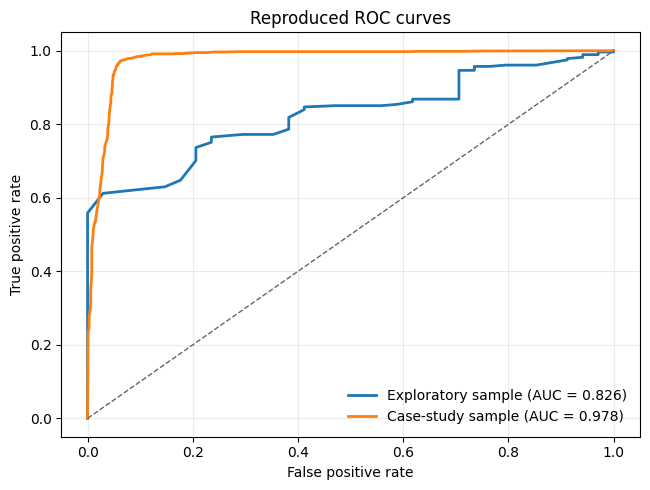
\includegraphics[width=0.95\textwidth]{../figures/roc_curves.png}
    \caption{Courbes ROC reproduites pour l'échantillon exploratoire et pour l'étude de cas canonique. Le résultat de l'étude de cas constitue le principal résultat quantitatif de l'article.}
\end{figure}

\begin{table}[H]
\centering
\caption{Performance prédictive reproduite à partir de la reconstruction canonique MASLCE.}
\begin{tabularx}{\textwidth}{p{5.0cm} c c c c c c}
\toprule
\textbf{Évaluation} & \textbf{Exact.} & \textbf{Précis.} & \textbf{Rappel} & \textbf{F1} & \textbf{Spécif.} & \textbf{AUC} \\
\midrule
Échantillon exploratoire, script archivé & 0,873 & 0,914 & 0,947 & 0,930 & 0,265 & 0,826 \\
Échantillon exploratoire, rerun nettoyé & 0,879 & 0,912 & 0,957 & 0,934 & 0,235 & 0,841 \\
Étude de cas, script canonique & 0,954 & 0,940 & 0,975 & 0,957 & 0,930 & 0,978 \\
Validation sur les extrêmes confirmés, sous-ensemble de l'étude de cas & 0,994 & 1,000 & 0,889 & 0,941 & 1,000 & 0,999 \\
\bottomrule
\end{tabularx}
\end{table}

\subsection{Composition indiciaire dans l'échantillon large}
Les distributions reproduites dans l'étude de cas soutiennent également la pertinence substantielle des trois indicateurs. Les cas à risque défavorable sont plus fortement associés à des prix fortement suspects, à des contenus dupliqués ou très similaires, et à des profils récents ou opaques que les cas à risque acceptable. Inversement, les profils anciens se concentrent davantage parmi les annonces acceptables.

\begin{figure}[H]
    \centering
    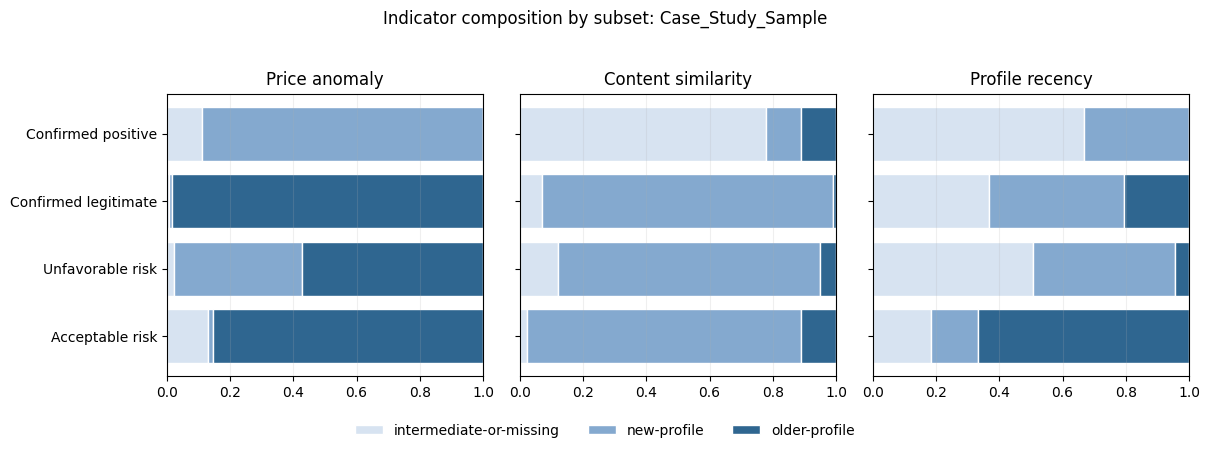
\includegraphics[width=0.98\textwidth]{../figures/case_indicator_distribution.png}
    \caption{Composition des indicateurs dans différents sous-ensembles du jeu de données canonique. Le sous-ensemble des cas positifs confirmés est réduit, mais il se concentre fortement dans les bandes de prix suspects et de contenu dupliqué.}
\end{figure}

Le petit nombre de cas positifs confirmés dans l'échantillon large constitue une limite, mais il reste informatif. Parmi ces cas extrêmes, le contenu dupliqué et les prix suspects sont fortement surreprésentés, tandis que les profils anciens sont absents. Cette structure ne démontre pas l'universalité du modèle ; elle confirme néanmoins la logique pratique des indicateurs.

\section{La contribution réelle du modèle}
Les professionnels appelés à évaluer cette recherche doivent se concentrer sur ce que le modèle apporte réellement, et non sur ce qu'une lecture trop ambitieuse voudrait lui faire dire. La contribution décisive n'est pas l'invention d'un pipeline d'apprentissage automatique inédit. Elle réside dans la mise en forme d'un cadre transparent, auditable et opérationnellement signifiant pour identifier suffisamment tôt des annonces à risque élevé.

Cette contribution comporte quatre dimensions.

\textbf{Premièrement, le modèle traduit un savoir de terrain en écran de détection répétable.} Les enquêteurs et les analystes travaillent souvent à partir de signaux récurrents, mais ces signaux sont rarement formalisés de manière transmissible. Le modèle MASLCE convertit une suspicion tacite en structure de scoring documentée.

\textbf{Deuxièmement, le modèle conserve un point de décision humain.} Parce que l'indice est interprétable, il ne place pas les professionnels dans une relation de confiance aveugle à la machine. Une annonce signalée peut être revue, contextualisée puis soit escaladée, soit rejetée avec motivation. Cet avantage pratique est majeur lorsque les faux positifs peuvent avoir des conséquences réputationnelles, commerciales ou juridiques.

\textbf{Troisièmement, le modèle favorise l'auditabilité.} Le score peut être conservé avec les valeurs des indicateurs, la version des seuils et les notes de l'analyste. Il devient alors possible de documenter les faux positifs récurrents, les dérives de calibration et les nouveaux schémas de fraude qui échappent encore au modèle. L'auditabilité n'est pas seulement une garantie de redevabilité ; elle est une condition d'apprentissage collectif.

\textbf{Quatrièmement, le modèle est opérationnellement flexible.} Il peut servir à la priorisation de files de revue, à des systèmes d'alerte, à une modération préliminaire, à une veille orientée renseignement, ou à la coordination public--privé. Sa valeur ne dépend pas d'un scénario unique d'implantation.

\begin{figure}[H]
    \centering
    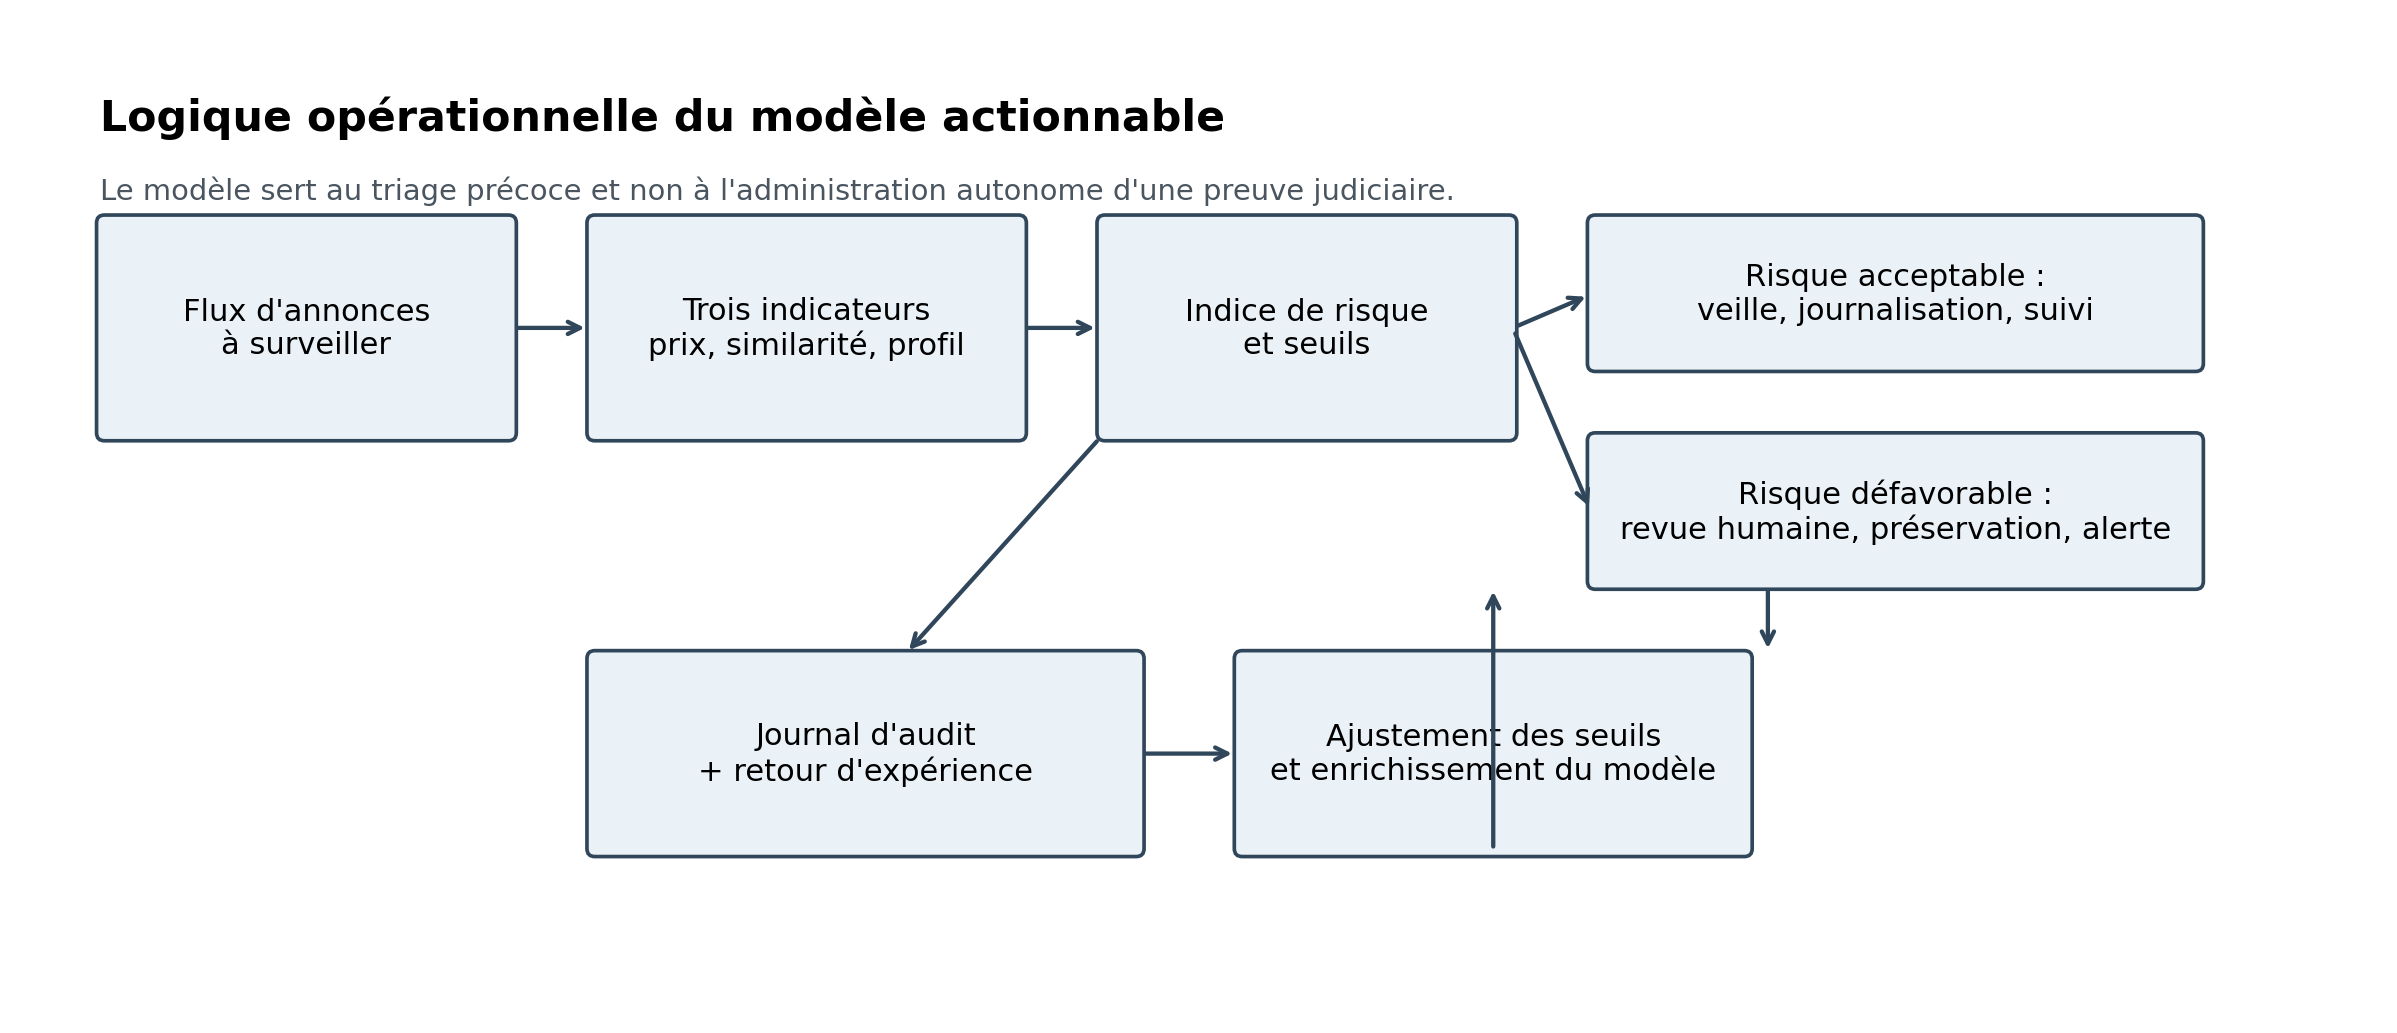
\includegraphics[width=0.96\textwidth]{../figures/operational_workflow_fr.png}
    \caption{Logique opérationnelle du modèle actionnable lorsqu'il est déployé comme système de triage du risque et non comme moteur autonome d'administration de la preuve.}
\end{figure}

C'est pourquoi cet article retient une formulation précise : la recherche est prête pour un examen par un jury de publication lorsqu'on définit sa contribution comme un modèle de triage proactif du risque au service de la prévention, de la modération, de la préservation des traces et de la coordination précoce. Dans ces termes, le modèle est à la fois plus modeste et plus crédible qu'une revendication de classification universelle de la fraude.

\section{Intégrité, reproductibilité et limites}
Un article prêt pour examen doit exposer non seulement les forces de l'étude, mais aussi les problèmes d'intégrité identifiés lors de la reconstruction.

\subsection{Ce qui se reproduit correctement}
Les principaux totaux descriptifs des jeux de données canoniques se reproduisent proprement, et le bloc métrique central de l'étude de cas résiste bien à la relecture et au rerun. C'est important, car cela montre que le résultat quantitatif principal n'est pas un artefact fragile issu d'un seul script défaillant. La séquence mixte est également cohérente : les catégories qualitatives et les indicateurs quantitatifs s'alignent nettement.

\subsection{Ce qui exige prudence ou correction}
L'audit a toutefois identifié plusieurs points qui importent pour une interprétation de qualité publication.

Le premier point est la \textbf{dérive de versions}. L'archive contient plusieurs copies et générations de scripts et de données. Une canonisation des fichiers était donc nécessaire avant de pouvoir énoncer des affirmations stables.

Le deuxième point est une \textbf{erreur de restitution des matrices de confusion dans le mémoire}. La reconstruction suggère que certaines tables publiées inversent faux positifs et faux négatifs, alors même que les autres métriques restent cohérentes. Il s'agit d'un problème de reporting, pas d'un effondrement du résultat sous-jacent, mais il doit être reconnu.

Le troisième point est la présence d'une \textbf{variable de fuite prédictive indésirable} dans l'un des scripts exploratoires. Le modèle exploratoire archivé utilisait un code d'état manuel qui ne serait pas disponible dans un contexte de déploiement propre. Le retrait de cette variable laisse subsister une performance de même ordre, ce qui est rassurant ; son inclusion initiale n'en demeure pas moins méthodologiquement problématique.

Le quatrième point concerne la \textbf{qualité du code ancien}. Certains scripts de similarité de première génération sont analytiquement invalides ou dépassés, et des fichiers de scraping anciens contenaient des éléments sensibles de type identifiants. Ces scripts ont été exclus du compendium final et ne doivent pas être redistribués ni exécutés dans un cadre de reproduction.

Le cinquième point tient à la \textbf{validité externe limitée}. La base probatoire reste centrée sur Facebook Marketplace et sur une famille de produits dont le prix de référence est relativement facile à estimer. L'article doit donc résister à toute prétention d'universalité.

\subsection{Faux positifs et ressemblances commerciales}
L'un des résultats les plus intéressants du mémoire est que certains cas fortement signalés n'étaient pas frauduleux mais commercialement agressifs. Des annonces légitimes publiées par des intermédiaires commerciaux peuvent ressembler à des fraudes parce qu'elles recourent à du contenu répété, à des profils récents et à une forte réplication promotionnelle. Pour les professionnels, ce constat n'est pas un embarras ; c'est une leçon opérationnelle. Le modèle détecte une \emph{structure de suspicion}, pas une vérité pénale métaphysique. C'est précisément la raison pour laquelle un point de revue humaine demeure indispensable.

\begin{table}[H]
\centering
\caption{Appréciation synthétique de la recherche au regard d'un jury de publication.}
\begin{tabularx}{\textwidth}{p{2.9cm} p{2.2cm} Y Y}
\toprule
\textbf{Critère} & \textbf{Appréciation} & \textbf{Motif principal} & \textbf{Implication pour la publication} \\
\midrule
Originalité & Forte & L'originalité réside dans la formalisation opérationnelle d'un savoir praticien plutôt que dans la nouveauté algorithmique. & Bonne adéquation avec une revue appliquée de criminologie ou de cybercrime. \\
Cohérence mixte & Forte & Les résultats thématiques nourrissent clairement le modèle indiciaire utilisé ensuite quantitativement. & Soutient une publication comme étude exploratoire sérieuse. \\
Force quantitative & Forte en interne & Le bloc métrique de l'étude de cas se reproduit correctement sur données canoniques. & Les résultats sont publiables si l'on décrit bien la nature interne de la cible de risque. \\
Validité externe & Limitée & Spécificité de plateforme et de produits. & Les prétentions doivent rester pilotées et contextuelles. \\
Reproductibilité & Moyenne à forte après audit & La reconstruction exige une canonisation et une correction de certaines incohérences. & Publication recommandée avec note explicite sur la reproductibilité. \\
Usabilité opérationnelle & Très forte & La logique indiciaire est transparente, auditable et compatible avec une revue humaine. & Contribution majeure pour un lectorat professionnel. \\
Préparation globale & Positive sous conditions de cadrage & Le travail est le plus robuste comme modèle de triage proactif du risque. & Prêt pour examen par un jury de publication dans ces termes. \\
\bottomrule
\end{tabularx}
\end{table}

\section{Trois implications pour la pratique et pour la recherche}
L'un des objectifs explicites de cet article est d'explorer trois implications majeures pour la pratique et pour la recherche. Elles forment ensemble le prolongement le plus utile de la contribution centrale.

\subsection{Implication 1 : passer d'une logique de plainte à une logique de triage du risque}
Pour la pratique, la première implication concerne la posture opérationnelle. La fraude par petites annonces ne devrait pas être traitée exclusivement comme un problème aval de réception de plaintes. Le modèle MASLCE montre qu'il est possible de signaler en amont des annonces à risque élevé au moyen d'indices publics compréhensibles et relativement peu coûteux à observer. Cela ne supprime pas le besoin d'enquête réactive ; cela améliore le point à partir duquel l'enquête réactive peut commencer.

Pour la recherche, la même implication invite à déplacer les critères d'évaluation. Il ne suffit pas de demander si un modèle prédit des labels finaux. Il faut aussi examiner s'il améliore le triage précoce, la gestion de charge analytique, la conservation de traces et la capacité préventive. Ces variables sont cruciales dans des settings réels de sécurité, mais elles sont souvent négligées par les évaluations strictement benchmarkées.

\subsection{Implication 2 : privilégier la transparence et l'auditabilité face à l'optimisation opaque}
Pour la pratique, la deuxième implication est une leçon de discipline méthodologique. Dans de nombreux environnements sensibles, un modèle légèrement moins spectaculaire mais clairement explicable peut être plus utile qu'une boîte noire plus performante. Le modèle MASLCE rappelle qu'en matière de fraude, la légitimité opérationnelle dépend de l'explicabilité. Les superviseurs, les partenaires de plateforme et les réviseurs extérieurs doivent pouvoir comprendre pourquoi une annonce a été escaladée.

Pour la recherche, cette implication plaide pour une valorisation accrue de l'auditabilité, des journaux décisionnels et de la gouvernance des seuils. La reproductibilité n'est pas un supplément de présentation ; elle fait partie intégrante de la validité lorsque le résultat doit soutenir l'action de sécurité.

\subsection{Implication 3 : penser le modèle comme un objet de coordination interinstitutionnelle}
Pour la pratique, la troisième implication est institutionnelle. La fraude par petites annonces se situe dans un espace fragmenté : police, plateformes, acteurs de prévention, régulateurs et consommateurs n'agissent ni au même moment ni avec les mêmes seuils. Un modèle auditable devient alors un support de coordination. Il permet de parler une langue commune du risque, même lorsque les mandats divergent.

Pour la recherche, cette implication ouvre des travaux sur la circulation d'indicateurs entre institutions, sur les conditions de partage public--privé, sur l'adaptation de seuils selon les usages, et sur l'articulation entre signaux publics et données propriétaires. La question n'est plus seulement : \emph{le modèle détecte-t-il ?} La question devient : \emph{comment un modèle explicable améliore-t-il la coordination d'un écosystème de sécurité ?}

\callout{\textbf{Lecture synthétique des trois implications.} Le modèle MASLCE soutient un passage de la plainte à l'anticipation, une préférence méthodologique pour l'explicabilité plutôt que pour l'opacité, et une mise en circulation du raisonnement de risque entre acteurs hétérogènes.}

\section{Scénarios illustratifs de déploiement}
Pour des professionnels, un bon article n'est pas seulement un récit de résultats ; il doit aussi montrer comment un modèle pourrait être intégré à des usages concrets. Les scénarios suivants ne valent pas comme prescriptions universelles. Ils illustrent les formes raisonnables que pourrait prendre un déploiement pilote.

\subsection{Modération préliminaire côté plateforme}
Une plateforme de petites annonces peut utiliser le modèle comme filtre de revue prioritaire. Les annonces les plus fortement signalées sont orientées vers un contrôle humain renforcé, tandis que les annonces à risque faible restent dans le flux normal. L'intérêt du modèle est alors double : il améliore la priorisation et il laisse une trace explicite des raisons ayant motivé la revue.

\subsection{Veille de renseignement dans un service spécialisé}
Un service de police ou de renseignement criminel peut utiliser le modèle pour repérer des grappes d'annonces fortement similaires, des profils nouveaux associés à des contenus dupliqués, ou des dynamiques de repost répétées sur plusieurs secteurs géographiques. Ici, la valeur du modèle ne tient pas seulement au classement unitaire, mais à sa capacité à produire des signaux de série.

\subsection{Prévention et signalétique publique}
Une institution de prévention ou une plateforme peut traduire certains signaux en signalétique visible pour les usagers : prix très inférieur au marché, texte fortement dupliqué, profil récent. Une telle approche ne remplace pas la modération ; elle peut néanmoins diminuer le nombre d'interactions dangereuses en amont.

\subsection{Appui à la conservation de traces}
Dans un environnement où les annonces disparaissent vite, le modèle peut servir d'interrupteur analytique : lorsqu'un certain seuil est dépassé, la capture technique d'éléments non sensibles et la journalisation d'un identifiant de listing deviennent prioritaires. Le bénéfice est alors moins la détection instantanée que la réduction de la perte future d'information.

\begin{longtable}{p{3.1cm} p{4.2cm} p{3.4cm} p{4.2cm}}
\caption{Exemples de déploiement pilote à destination de professionnels.}\\
\toprule
\textbf{Contexte} & \textbf{Usage du modèle} & \textbf{Seuil d'action prioritaire} & \textbf{Bénéfice principal} \\
\midrule
\endfirsthead
\toprule
\textbf{Contexte} & \textbf{Usage du modèle} & \textbf{Seuil d'action prioritaire} & \textbf{Bénéfice principal} \\
\midrule
\endhead
Plateforme de petites annonces & Priorisation de la revue humaine d'annonces nouvelles & Score élevé ou accumulation d'indicateurs forts & Réduction du délai entre publication et revue, amélioration de l'explicabilité des décisions de modération \\
Service spécialisé police / cyber & Veille, repérage de grappes, conservation de traces & Répétition d'alertes sur contenus ou profils liés & Préservation d'éléments utiles avant disparition des annonces \\
Prévention institutionnelle & Signalétique ou messages d'alerte aux usagers & Combinaison de prix suspects et de profils récents & Diminution des prises de contact dangereuses et amélioration de la vigilance publique \\
Cellule de coopération public--privé & Échange d'indicateurs et calibration de seuils & Répétition multi-sites ou multi-zones & Langage commun du risque entre acteurs aux mandats distincts \\
\bottomrule
\end{longtable}

\section{Conditions d'un usage responsable}
L'utilité d'un modèle de triage dépend de la discipline de son usage. Trois conditions méritent d'être explicitées.

La première est la \textbf{séparation claire entre risque et preuve}. Un signalement défavorable n'est ni une qualification pénale ni une vérité définitive. C'est une raison structurée d'examiner davantage.

La deuxième est la \textbf{présence d'une revue humaine documentée}. Tout déploiement responsable doit prévoir des motifs de confirmation, d'infirmation et de reclassement. C'est cette couche humaine qui permet d'absorber les cas d'agressivité commerciale légitime et de corriger les faux positifs.

La troisième est la \textbf{gouvernance des seuils et des journaux}. Les seuils utilisés, les versions du modèle et les décisions prises doivent être historisés. Sans cela, il devient impossible de comprendre l'évolution des faux positifs, des faux négatifs et des zones d'angle mort.

Pour un jury de publication, ces conditions sont importantes car elles évitent deux dérives symétriques : l'idéalisation de la détection automatique et la disqualification injustifiée du modèle au motif qu'il ne fournirait pas une preuve autonome. Le bon niveau de lecture est intermédiaire : un outil de triage transparent capable d'améliorer la prévention, la priorisation et la coordination.

\section{Conclusion}
Le projet MASLCE démontre qu'il est possible de construire un modèle actionnable de détection proactive de la fraude à partir de signaux simples, compréhensibles et auditables. Sa force ne vient pas d'une sophistication algorithmique extraordinaire ; elle vient de la transformation méthodique d'un savoir de terrain en un dispositif de triage du risque qui reste lisible pour les professionnels.

La reconstruction documentée montre que le résultat quantitatif principal tient correctement après canonisation de l'archive. Elle montre également que plusieurs limites doivent être assumées : base empirique spécifique, dérives de versions, erreurs de restitution dans certaines tables et présence initiale d'un prédicteur indésirable dans un script exploratoire. Ces limites n'annulent pas la contribution ; elles précisent son régime de validité.

Sur ces bases, l'article soutient que la recherche est prête pour un examen par un jury de publication à condition d'être présentée dans ses termes les plus solides : une méthode transparente, auditable et opérationnellement signifiante pour identifier plus tôt des annonces à risque élevé dans un contexte où la seule réaction institutionnelle demeure insuffisante. Pour les professionnels de la criminalité économique et de la cybercriminalité, cette contribution est loin d'être mineure. Elle propose non pas une promesse magique, mais un outil réaliste de priorisation, de prévention et de coordination.

\newpage

\section{Checklist professionnelle pour un pilote de déploiement}
\begin{longtable}{p{5.0cm} p{10.2cm}}
\caption{Checklist minimale pour un pilote d'usage responsable du modèle.}\\
\toprule
\textbf{Point de contrôle} & \textbf{Question à documenter avant déploiement} \\
\midrule
\endfirsthead
\toprule
\textbf{Point de contrôle} & \textbf{Question à documenter avant déploiement} \\
\midrule
\endhead
Finalité d'usage & Le modèle sert-il à l'alerte, à la priorisation de revue, à la conservation de traces, à la prévention, ou à une combinaison de ces fonctions ? \\
Définition de la cible & La distinction \emph{acceptable / défavorable} est-elle comprise comme catégorie de risque et non comme preuve pénale ? \\
Base de référence des prix & Les prix de marché utilisés sont-ils documentés, traçables et révisables selon les segments de produits ? \\
Revue humaine & Un opérateur identifié relit-il les cas signalés avant toute décision sensible ? \\
Journal d'audit & Les indicateurs, le score, la version des seuils et la décision humaine sont-ils conservés ? \\
Gestion des faux positifs & Une procédure existe-t-elle pour reclasser les cas relevant d'un comportement commercial agressif mais licite ? \\
Respect juridique & Les données utilisées sont-elles publiquement accessibles et le traitement respecte-t-il les contraintes légales applicables ? \\
Boucle de retour d'expérience & Les erreurs récurrentes sont-elles analysées afin de recalibrer les seuils et d'enrichir le modèle ? \\
Extension de recherche & En cas de succès du pilote, l'extension à d'autres produits ou plateformes préservera-t-elle les mêmes exigences d'audit et de documentation ? \\
\bottomrule
\end{longtable}

\newpage

\section{Trame minimale de journal d'analyse}
\begin{longtable}{p{4.2cm} p{11.0cm}}
\caption{Journal d'analyse minimal pour une annonce signalée.}\\
\toprule
\textbf{Champ} & \textbf{Fonction} \\
\midrule
\endfirsthead
\toprule
\textbf{Champ} & \textbf{Fonction} \\
\midrule
\endhead
Identifiant du listing et horodatage de capture & Permet de reconstituer précisément l'objet analysé et le moment de la revue. \\
Plateforme, produit, localisation & Replace l'annonce dans son segment de marché et son contexte de diffusion. \\
Référence de prix utilisée & Documente le benchmark ayant servi à juger le prix normal, sous-évalué ou fortement suspect. \\
Éléments de similarité & Indique si l'annonce réemploie un gabarit connu, duplique une annonce ou présente seulement une proximité partielle. \\
Éléments relatifs au profil & Consigne l'âge visible du compte, les absences d'information et la manière dont elles ont été interprétées. \\
Score total et bande de risque & Conserve le score, la bande de risque et la version du seuil appliqué. \\
Décision du relecteur humain & Confirme, infirme, reclasse en pratique commerciale agressive ou escalade pour approfondissement. \\
Justification synthétique & Oblige à motiver la décision, surtout en cas d'override du score initial. \\
Action engagée & Journalise le type d'action : avertissement, préservation, transmission, veille, clôture. \\
Issue ultérieure & Quand elle est connue, enregistre si le cas s'est révélé frauduleux, non frauduleux ou utile à la recalibration du modèle. \\
\bottomrule
\end{longtable}

\newpage

\section{Bandes de risque et niveaux d'action recommandés}
Le mémoire d'origine utilisait une lecture graduée de l'indice avant la simplification en \emph{acceptable} versus \emph{défavorable}. Pour un usage professionnel, cette granularité intermédiaire reste utile, car toutes les alertes n'appellent pas le même niveau de réponse.

\begin{longtable}{p{2.1cm} p{2.8cm} p{3.7cm} p{6.1cm}}
\caption{Lecture opérationnelle des bandes d'indice pour un déploiement préventif.}\\
\toprule
\textbf{Bande} & \textbf{Lecture pratique} & \textbf{Action minimale} & \textbf{Commentaire professionnel} \\
\midrule
\endfirsthead
\toprule
\textbf{Bande} & \textbf{Lecture pratique} & \textbf{Action minimale} & \textbf{Commentaire professionnel} \\
\midrule
\endhead
3--4 & Accumulation faible de signaux & Journalisation simple ou veille légère & Insuffisant pour une action intrusive sans contexte complémentaire ; utile pour la surveillance de motifs émergents. \\
5 & Seuil frontière & Relecture secondaire & Point important de calibration, car de nombreuses erreurs de seuil apparaissent autour de cette zone. \\
6--7 & Suspicion marquée & Revue prioritaire ou modération renforcée & Suffisamment fort pour une attention préventive, sans être encore assimilable à une preuve. \\
8--9 & Accumulation très forte de signaux & Préservation, revue rapide, éventuelle alerte & Catégorie de haute priorité à lire comme triage renforcé plutôt que comme démonstration autonome. \\
Répétition de grappes & Motif systémique au-delà du score unitaire & Veille structurée et coordination & La répétition sur de multiples annonces peut justifier une réponse même si chaque annonce reste individuellement incomplète. \\
\bottomrule
\end{longtable}

\newpage

\section{Critères d'appropriation institutionnelle}
Pour un lectorat professionnel, la question finale n'est pas uniquement de savoir si le modèle fonctionne, mais s'il peut être approprié sans générer d'effets pervers. L'expérience des dispositifs de détection montre qu'un score utile en laboratoire peut devenir contre-productif dès lors qu'il n'est ni gouverné, ni compris, ni révisé. Quatre conditions d'appropriation ressortent de la lecture croisée du mémoire, de la soutenance et du travail de reconstruction.

La première est la \textbf{stabilité de la doctrine d'usage}. Les acteurs doivent s'entendre sur ce que le score autorise et sur ce qu'il n'autorise pas. Un score élevé peut légitimer une revue prioritaire, une conservation de traces, une vigilance renforcée ou une coopération plus rapide avec une plateforme ; il ne doit pas être interprété comme un mécanisme autonome de qualification pénale. Cette doctrine protège à la fois l'efficacité du dispositif et la sécurité juridique des acteurs qui l'utilisent.

La deuxième condition est la \textbf{formation minimale des utilisateurs}. Un modèle transparent n'est utile que si les opérateurs savent lire un faux positif, reconnaître un cas de commerce agressif mais licite, et documenter proprement un désaccord avec la sortie du modèle. Une formation courte mais structurée suffit souvent : rappel de la logique indiciaire, cas-types, zones d'incertitude, et bonnes pratiques de journalisation.

La troisième condition est la \textbf{maintenance de la boucle d'apprentissage}. Les fraudeurs adaptent rapidement leurs modes opératoires ; un modèle figé perd donc progressivement sa valeur. Cela implique non pas une refonte permanente, mais un entretien régulier : revue des erreurs, recalibrage de certains seuils, ajout de nouveaux signaux lorsque les comportements changent, et documentation stricte de chaque modification.

La quatrième condition est la \textbf{compatibilité avec l'écosystème institutionnel}. Un dispositif de triage ne doit pas être conçu pour un acteur abstrait, mais pour des chaînes de décision concrètes. Si la plateforme, le service d'analyse, l'unité d'enquête ou l'acteur de prévention n'utilisent pas le même vocabulaire de risque, la promesse d'action précoce sera rapidement neutralisée. À l'inverse, un modèle simple et auditable peut devenir un support stable de coopération, précisément parce qu'il explicite ses critères et ses seuils.

En ce sens, l'enjeu principal du projet MASLCE dépasse la seule performance. Il touche à la capacité des institutions à intégrer un instrument de triage dans des workflows réels sans perdre ni la lisibilité de l'action ni la traçabilité des décisions. C'est cette compatibilité entre efficacité, explicabilité et gouvernance qui justifie, au fond, l'intérêt scientifique et professionnel de la recherche.


\newpage

\begin{thebibliography}{99}
\bibitem{alrousan2020} Al-Rousan, S., Abuhussein, A., Alsubaei, F., Collen, L., \& Shiva, S. (2020). Ads-Guard: Detecting scammers in online classified ads. \emph{2020 IEEE Symposium Series on Computational Intelligence}, 1492--1498.
\bibitem{alzghoul2024} Alzghoul, J. R., Abdallah, E. E., \& Al-khawaldeh, A. S. (2024). Fraud in online classified ads: Strategies, risks, and detection methods. \emph{Journal of Applied Security Research, 19}(1), 45--69.
\bibitem{aebi2022} Aebi, M., Caneppele, S., \& Molnar, L. (2022). \emph{Measuring cybercrime in Europe: The role of crime statistics and victimisation surveys}. Eleven.
\bibitem{avenier2007a} Avenier, M.-J., \& Schmitt, C. (2007a). Élaborer des savoirs actionnables et les communiquer à des managers. \emph{Revue française de gestion, 174}(5), 25--42.
\bibitem{avenier2007b} Avenier, M.-J., \& Schmitt, C. (2007b). \emph{La construction de savoirs pour l'action}. Paris: L'Harmattan.
\bibitem{benabdallah2023} Ben Abdallah, E., \& Boukadi, K. (2023). Online consumer review spam detection based on reinforcement learning and neural networks. \emph{Multimedia Tools and Applications, 83}(9), 25617--25641.
\bibitem{blais2006} Blais, M., \& Martineau, S. (2006). L'analyse inductive générale. \emph{Recherches qualitatives, 26}(2), 1--18.
\bibitem{costa2021} Costa, L. da F. (2021). Further generalizations of the Jaccard index. \emph{arXiv}.
\bibitem{dupont2014} Dupont, B. (2014). La régulation du cybercrime comme alternative à la judiciarisation : le cas des botnets. \emph{Criminologie, 47}(2), 179--201.
\bibitem{dupont2024} Dupont, B. (2024). \emph{La cybercriminalité : Approche écosystémique de l'espace numérique}. Paris: Armand Colin.
\bibitem{fortin2022} Fortin, M.-F., \& Gagnon, J. (2022). \emph{Fondements et étapes du processus de recherche : Méthodes quantitatives et qualitatives} (4\textsuperscript{e} éd.). Montréal: Chenelière.
\bibitem{jacquart2021} Jacquart, B., Schopfer, A., \& Rossy, Q. (2021). Mules financières : profils, recrutement et rôles de facilitateur pour les escroqueries aux fausses annonces. \emph{Revue internationale de criminologie et de police technique et scientifique, 74}(4), 409--426.
\bibitem{jaccard1902} Jaccard, P. (1902). Distribution comparée de la flore alpine dans quelques régions des Alpes occidentales et orientales. \emph{Bulletin de la Murithienne}, 81--92.
\bibitem{kumari2024} Kumari, A., \& Sharma, I. (2024). Mitigating malvertising threats through machine-learning classification. \emph{2024 International Conference on Advancements in Smart, Secure and Intelligent Computing}, 1--6.
\bibitem{leukfeldt2016} Leukfeldt, E. R., \& Yar, M. (2016). Applying routine activity theory to cybercrime. \emph{Deviant Behavior, 37}(3), 263--280.
\bibitem{leukfeldt2017} Leukfeldt, E. R., Lavorgna, A., \& Kleemans, E. R. (2017). Organised cybercrime or cybercrime that is organised? \emph{European Journal on Criminal Policy and Research, 23}(3), 287--300.
\bibitem{lopez2021} Lopez, B. E., Taylor, V. G., \& McGrath, J. G. (2021). Using forensic intelligence to combat serial and organised violent crimes. \emph{National Institute of Justice}.
\bibitem{malik2024} Malik, A. A., Azeem, W., \& Asad, M. (2024). Online shopping, cyber frauds and fraud prevention strategies. \emph{International Journal for Electronic Crime Investigation, 8}(1).
\bibitem{mancosu2020} Mancosu, M., \& Vegetti, F. (2020). What you can scrape and what is right to scrape. \emph{Social Media + Society, 6}(3).
\bibitem{mccormick2013} McCormick, A. M., \& Eberle, W. (2013). Discovering fraud in online classified ads. \emph{The Twenty-Sixth International FLAIRS Conference}.
\bibitem{mokhberi2024} Mokhberi, A., Huang, Y., Humbert, G., Obada-Obieh, B., Mehrabi Koushki, M., \& Beznosov, K. (2024). Trust, privacy, and safety factors associated with decision making in P2P markets based on social networks. \emph{Proceedings of the 2024 CHI Conference on Human Factors in Computing Systems}, 1--25.
\bibitem{nanath2023} Nanath, K., \& Olney, L. (2023). Crowdsourcing methods in enhancing machine learning for detecting online recruitment fraud. \emph{International Journal of Information Management Data Insights, 3}(1), 100167.
\bibitem{powers2020} Powers, D. M. W. (2020). Evaluation: from precision, recall and F-measure to ROC, informedness, markedness and correlation. \emph{arXiv}.
\bibitem{ribaux2023} Ribaux, O. (2023). \emph{De la police scientifique à la traçologie : Le renseignement par la trace}. Lausanne: PPUR.
\bibitem{rizka2024} Rizka, R. (2024). Legal protection for consumers who buy and sell used goods on Facebook. \emph{International Journal of Law and Policy, 2}(4).
\bibitem{rossy2020} Rossy, Q., \& Borisova, B. (2020). Escroqueries par Internet. In \emph{Cybercrimes et enjeux technologiques : contexte et perspectives} (pp. 227--250).
\bibitem{saumya2022} Saumya, S., \& Singh, J. P. (2022). Spam review detection using LSTM autoencoder. \emph{Electronic Commerce Research, 22}(1), 113--133.
\bibitem{shahariar2019} Shahariar, G. M., Biswas, S., Omar, F., Shah, F. M., \& Hassan, S. B. (2019). Spam review detection using deep learning. \emph{2019 IEEE 10th Annual Information Technology, Electronics and Mobile Communication Conference}, 27--33.
\bibitem{shaukat2023} Shaukat, M. W., Amin, R., Muslam, M. M. A., Alshehri, A. H., \& Xie, J. (2023). A hybrid approach for alluring ads phishing attack detection using machine learning. \emph{Sensors, 23}(19).
\bibitem{thomas2006} Thomas, D. R. (2006). A general inductive approach for analyzing qualitative evaluation data. \emph{American Journal of Evaluation, 27}(2), 237--246.
\bibitem{wall2015} Wall, D. S. (2015). The Internet as a conduit for criminal activity. In \emph{Information technology and the criminal justice system}.
\end{thebibliography}

\end{document}
